%%% Local Variables:
%%% mode: latex
%%% TeX-master: "../doc"
%%% coding: utf-8
%%% End:
% !TEX TS-program = pdflatexmk
% !TEX encoding = UTF-8 Unicode
% !TEX root = ../doc.tex
\section{Aufgabenstellung}
\label{sec:aufgabenstellung}
\begin{figure}[H]
  \centering
  
\includegraphics[page=1,scale=0.55]{../ressources/Aufgabenstellung.pdf}
\end{figure}
\begin{figure}[H]
  \centering

\includegraphics[page=2,scale=0.55]{../ressources/Aufgabenstellung.pdf}
\end{figure}


\section{Packages}
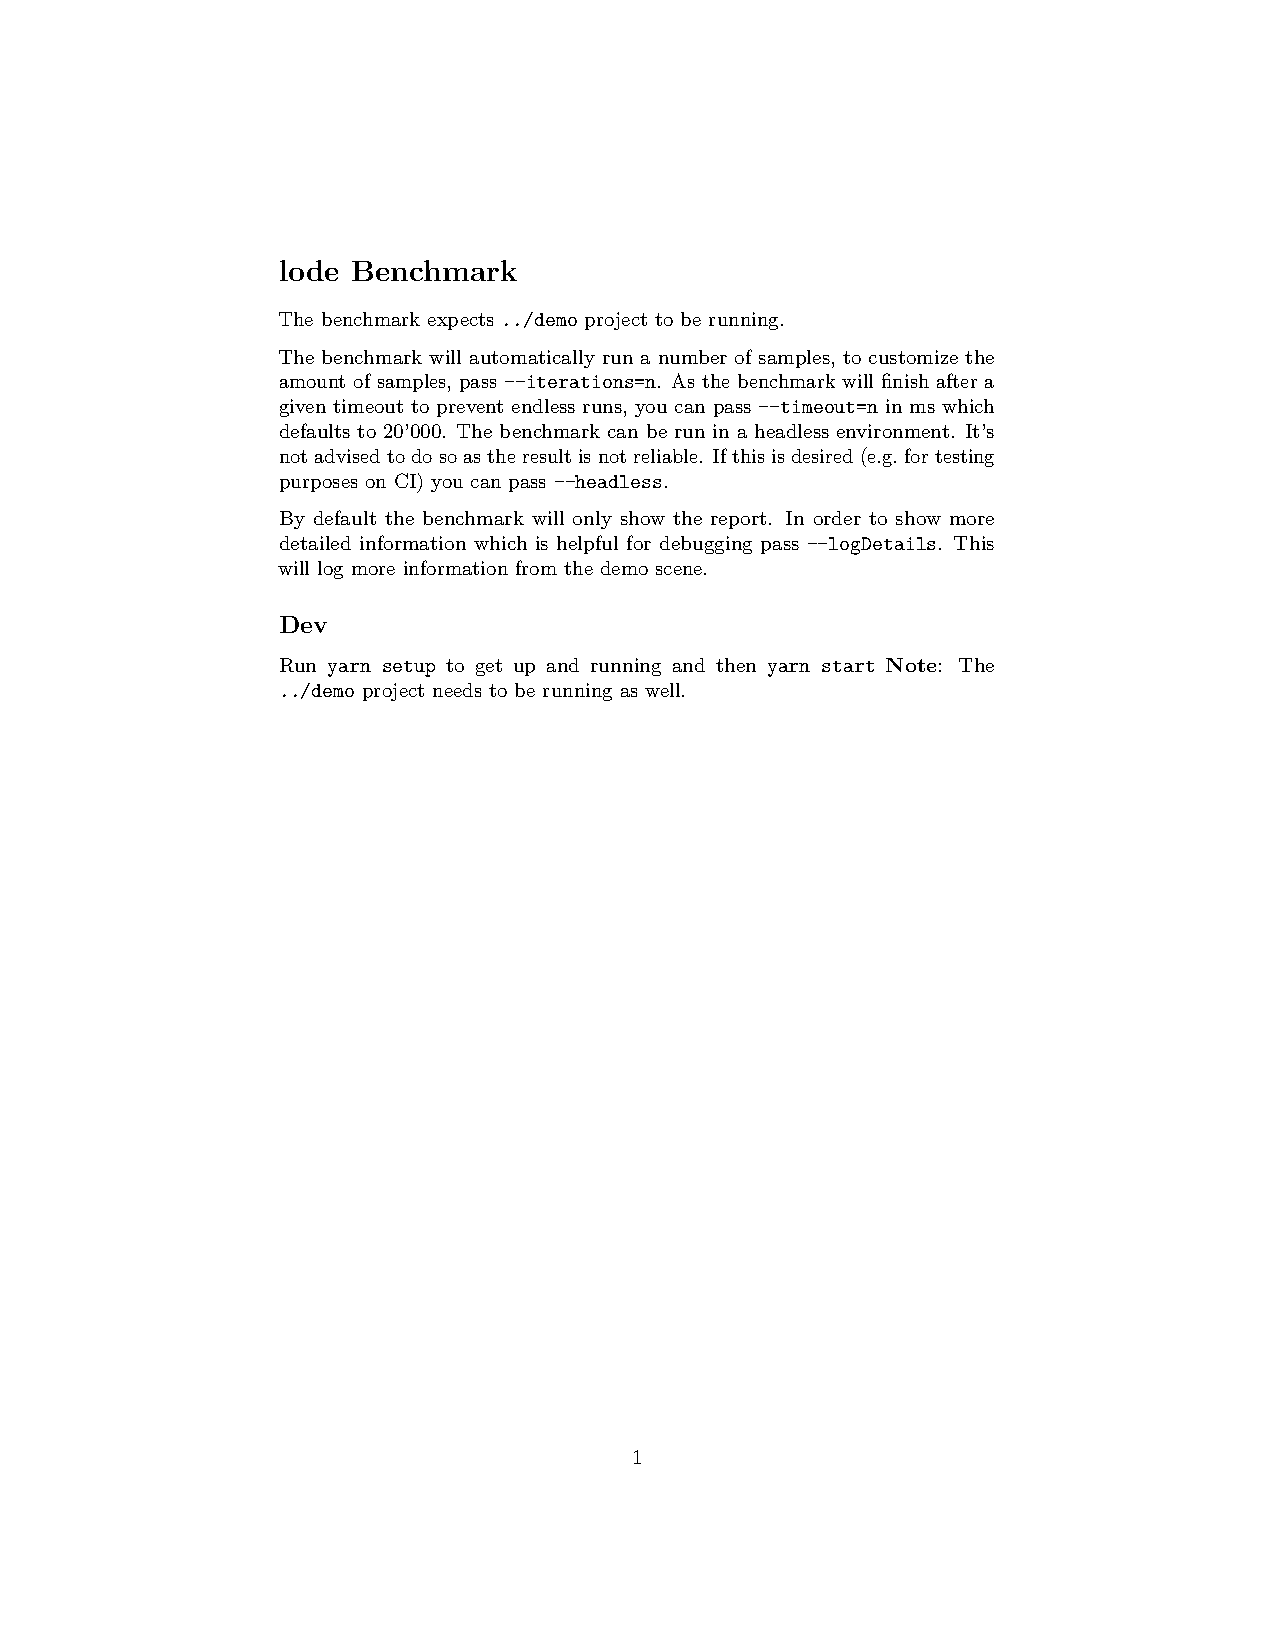
\includepdf[pagecommand={},scale=0.92,pages=-]{../ressources/packages/benchmark.pdf}
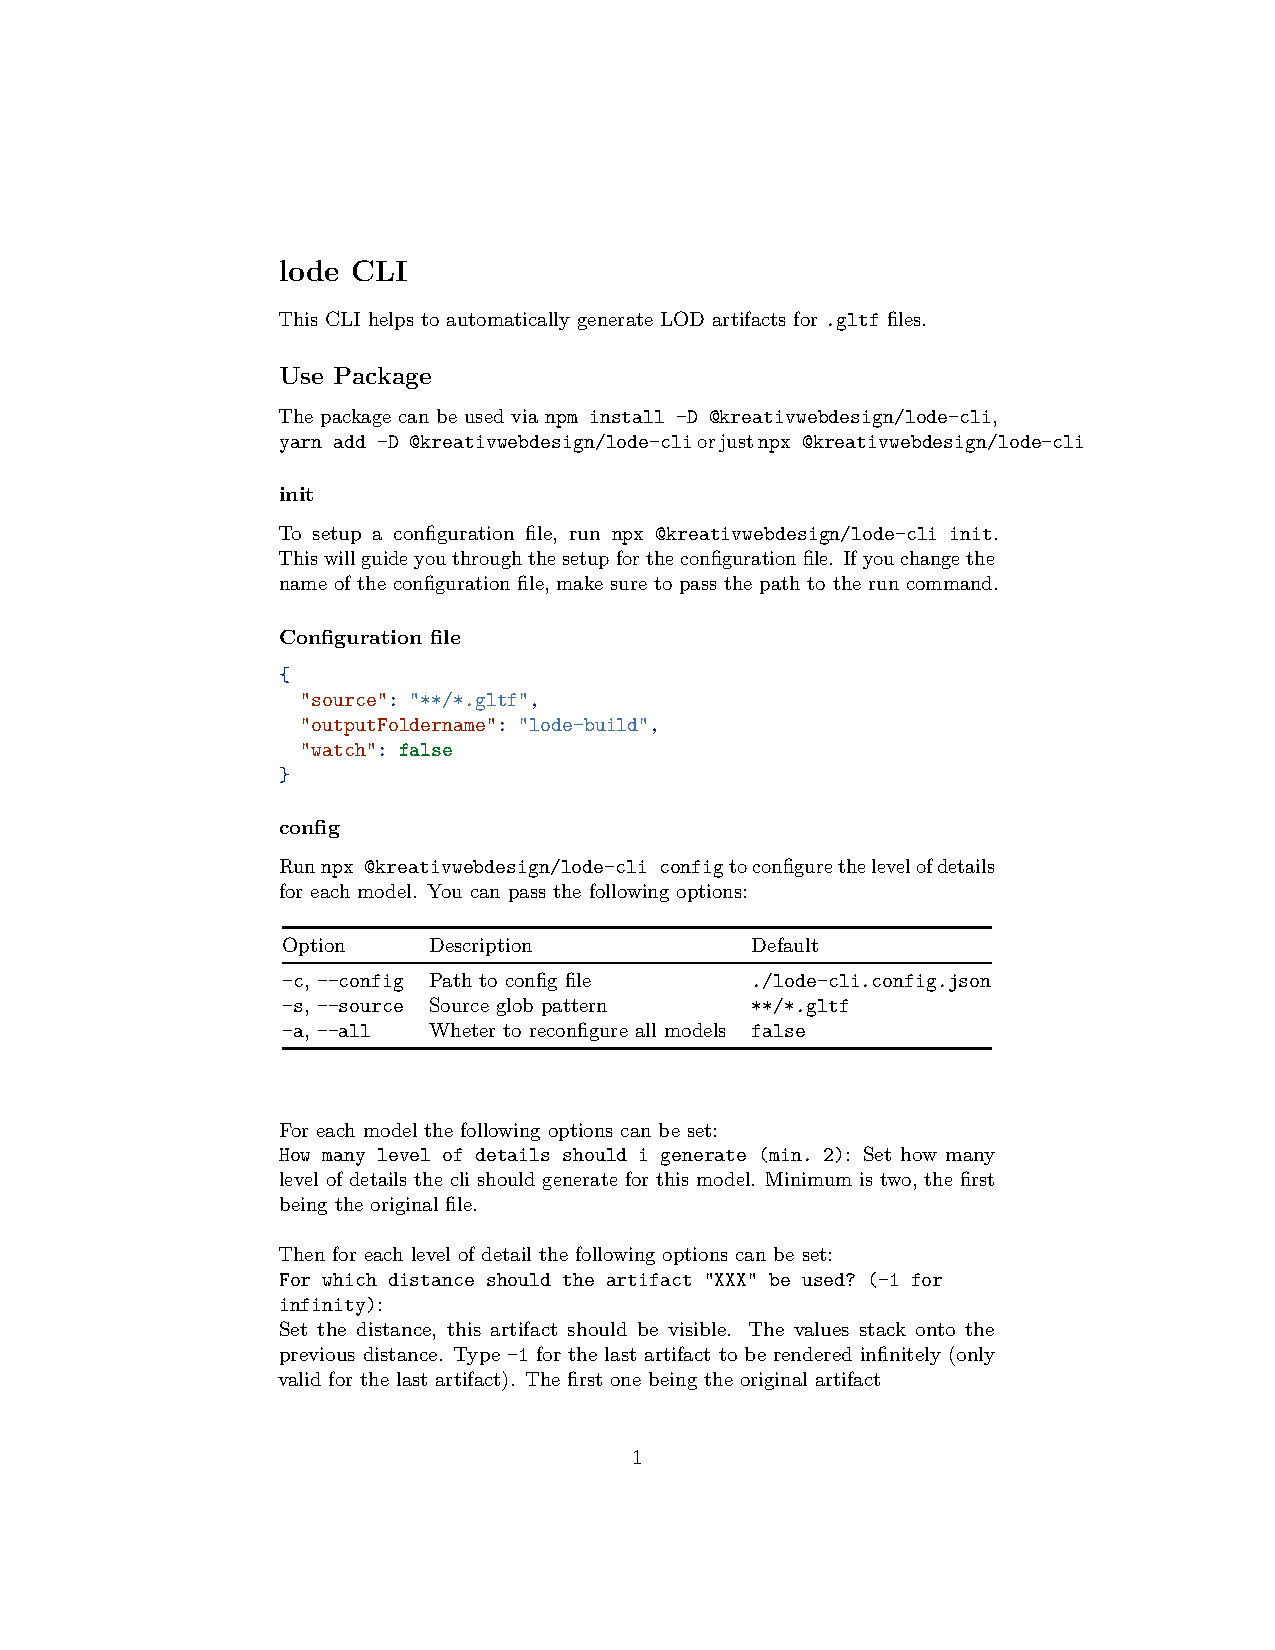
\includepdf[pagecommand={},scale=0.92,pages=-]{../ressources/packages/cli.pdf}
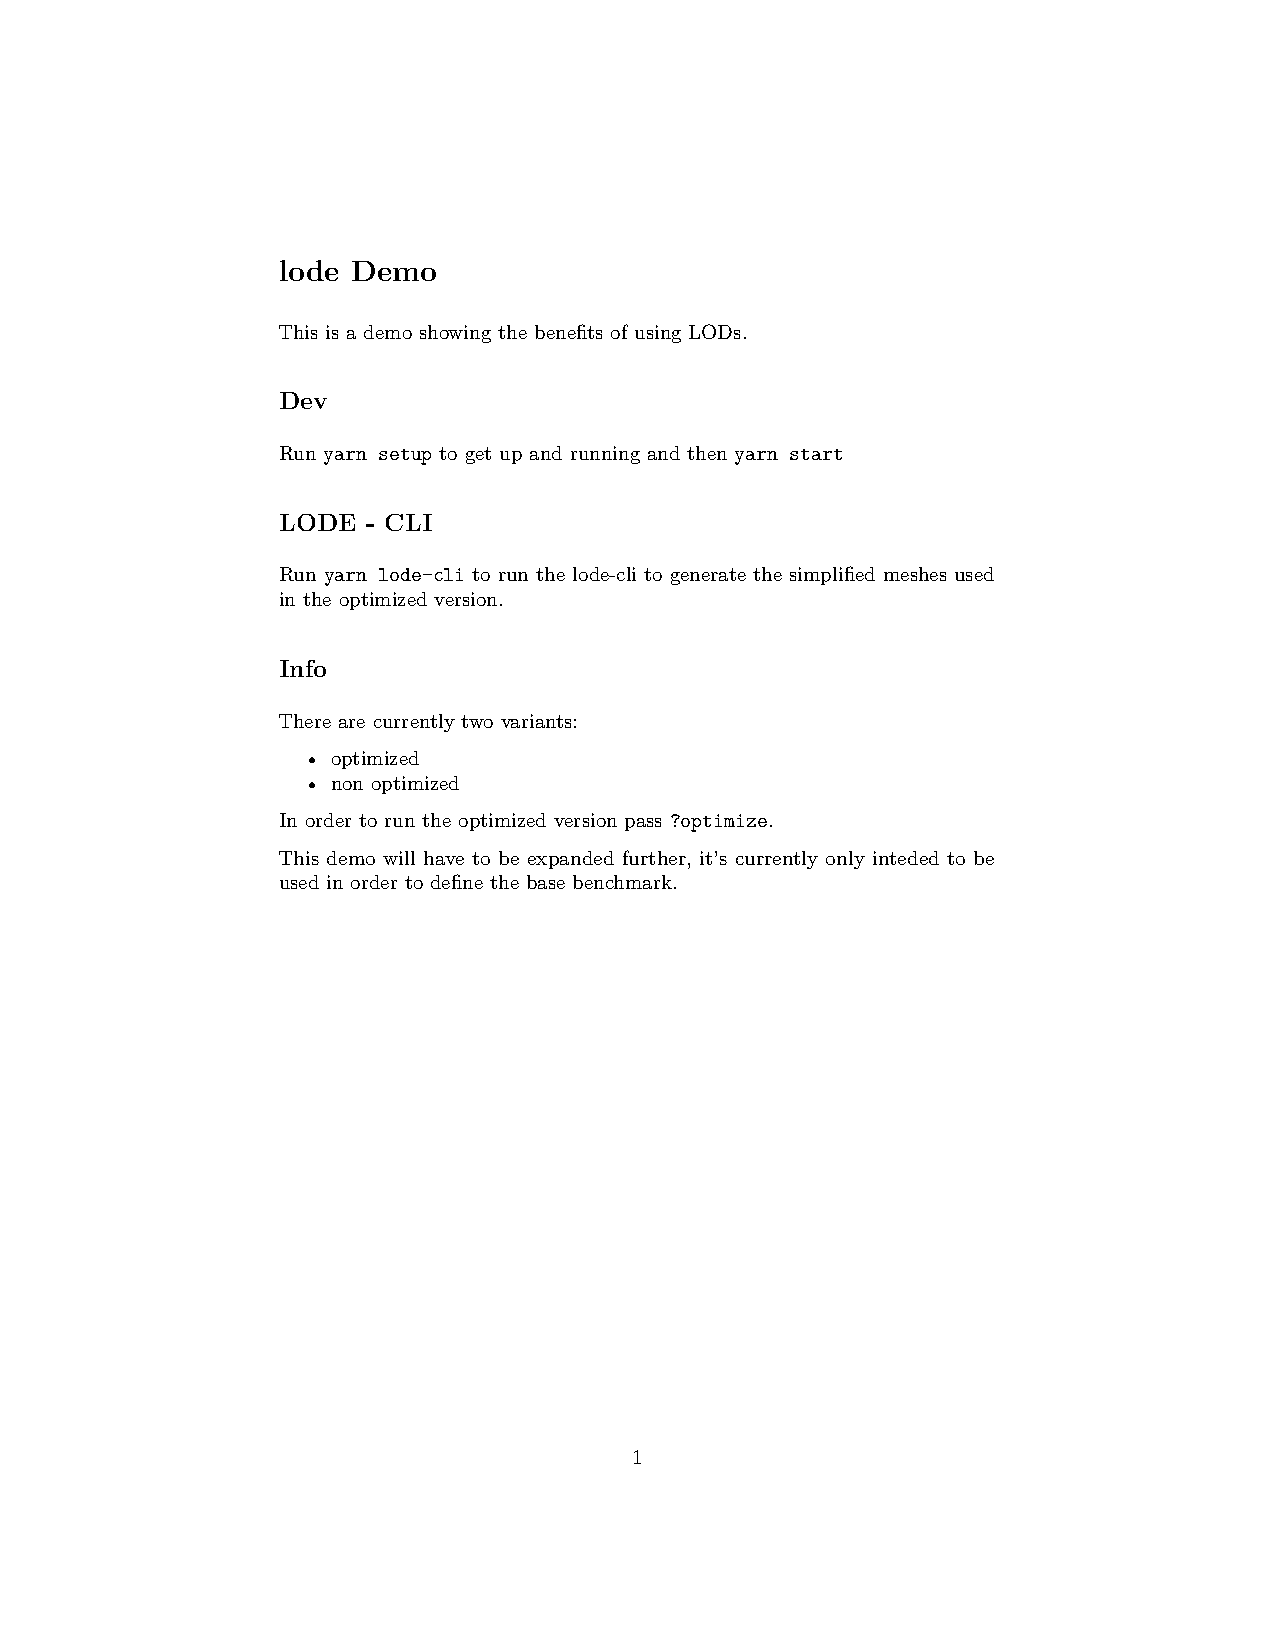
\includepdf[pagecommand={},scale=0.92,pages=-]{../ressources/packages/demo.pdf}
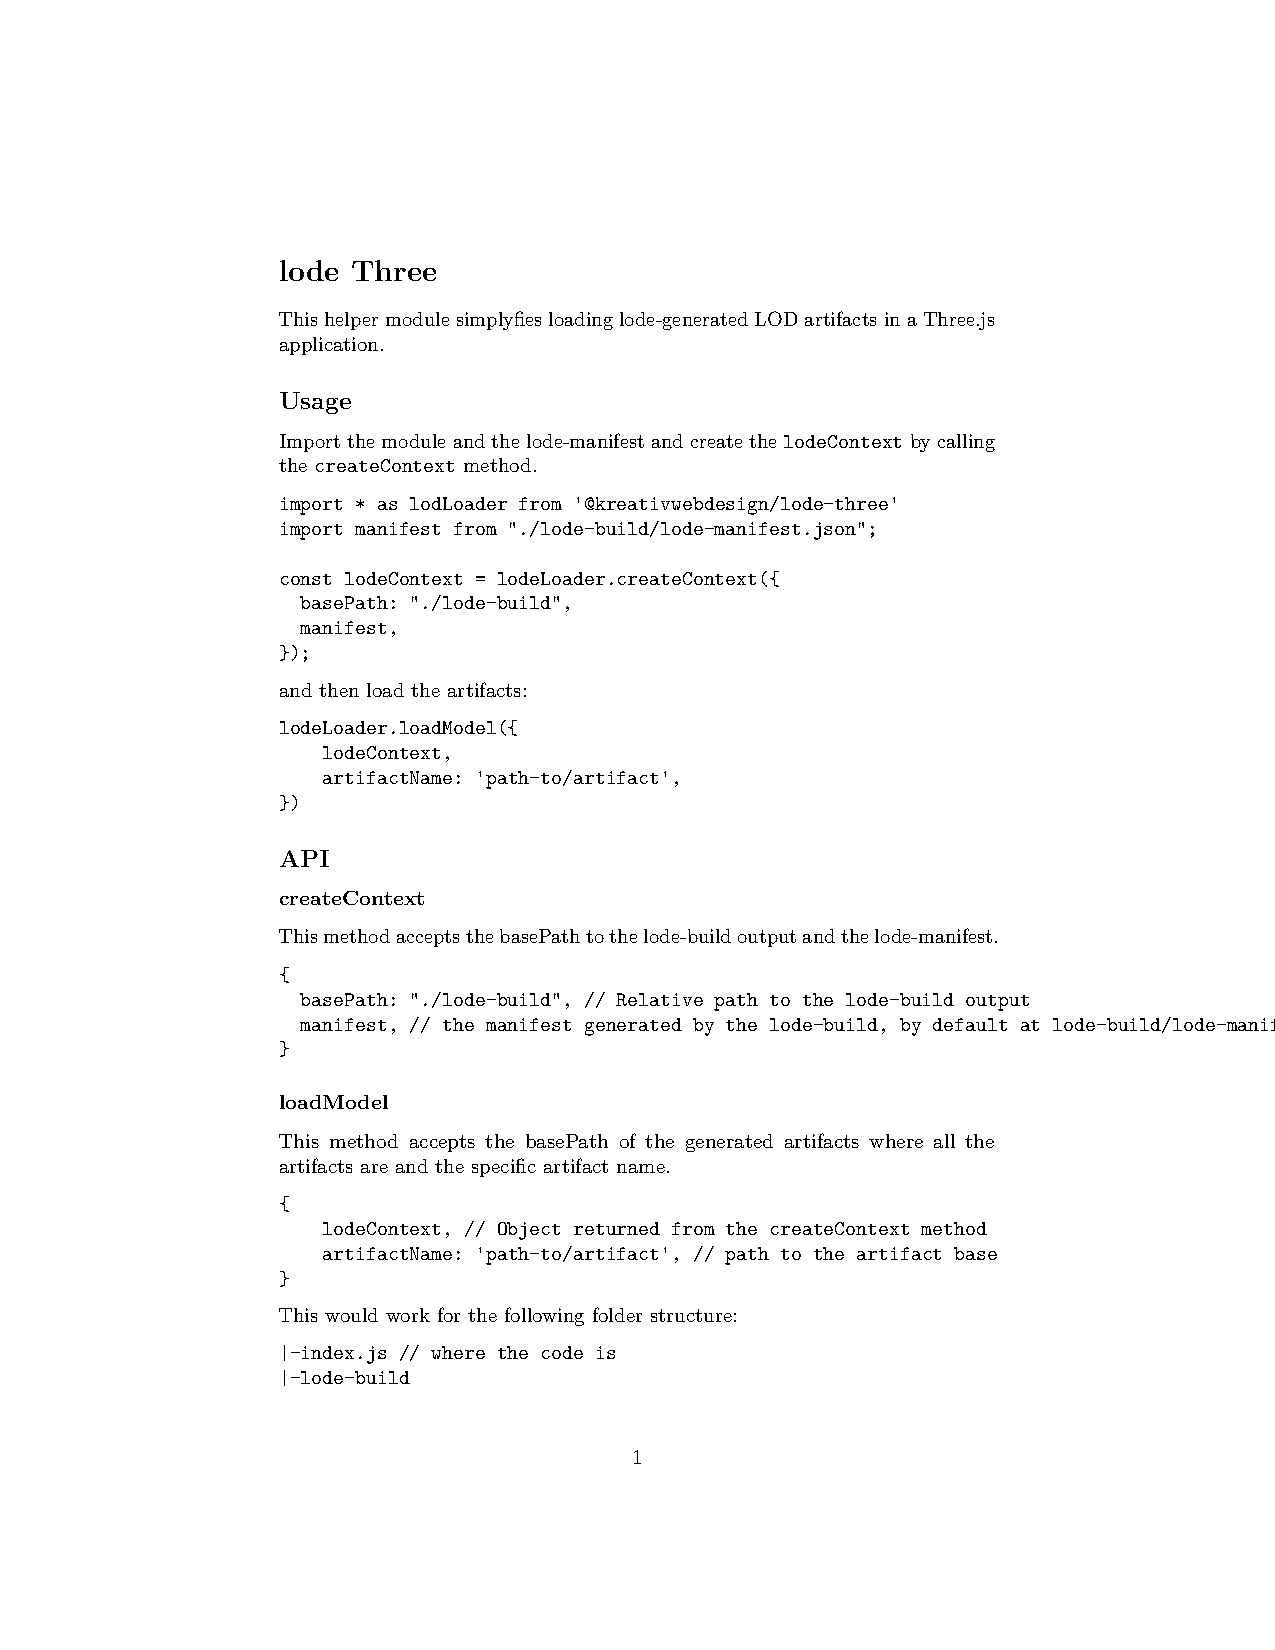
\includepdf[pagecommand={},scale=0.92,pages=-]{../ressources/packages/lode-three.pdf}
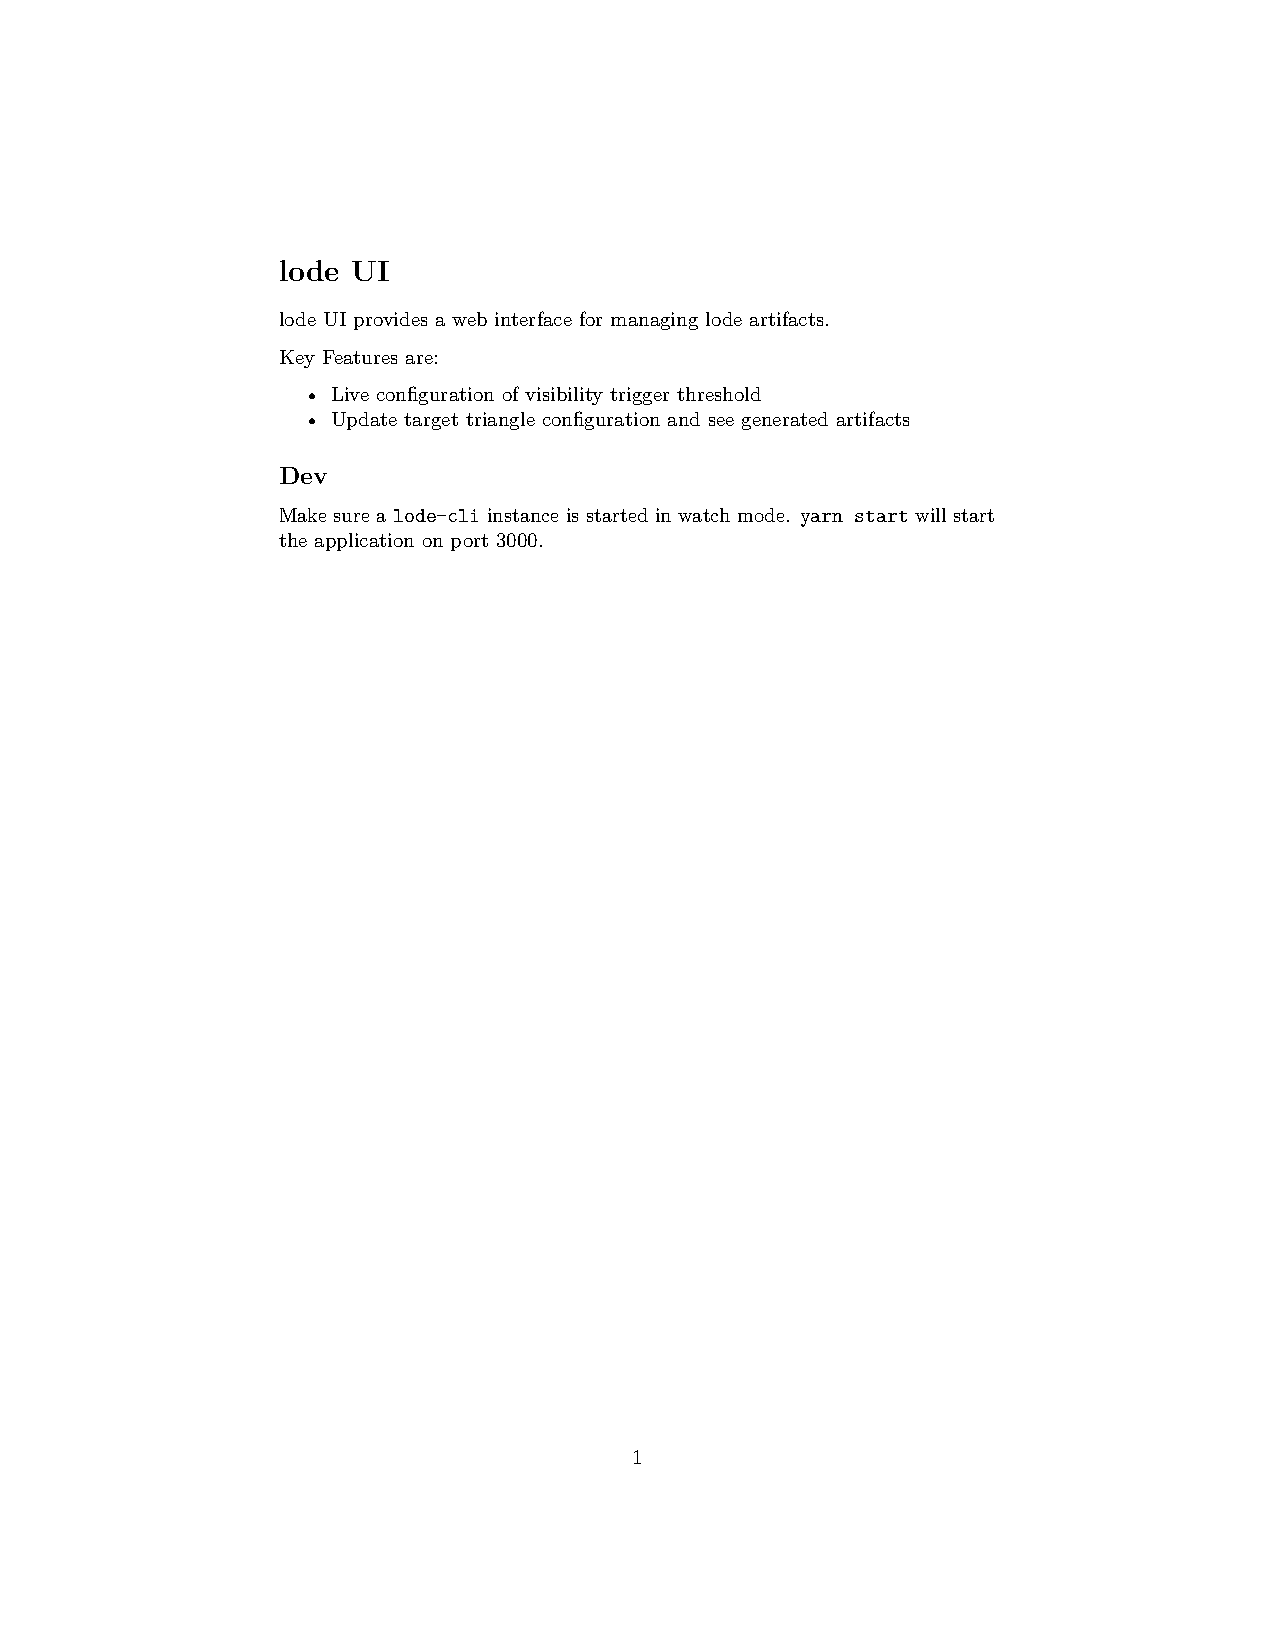
\includepdf[pagecommand={},scale=0.92,pages=-]{../ressources/packages/lode-ui.pdf}
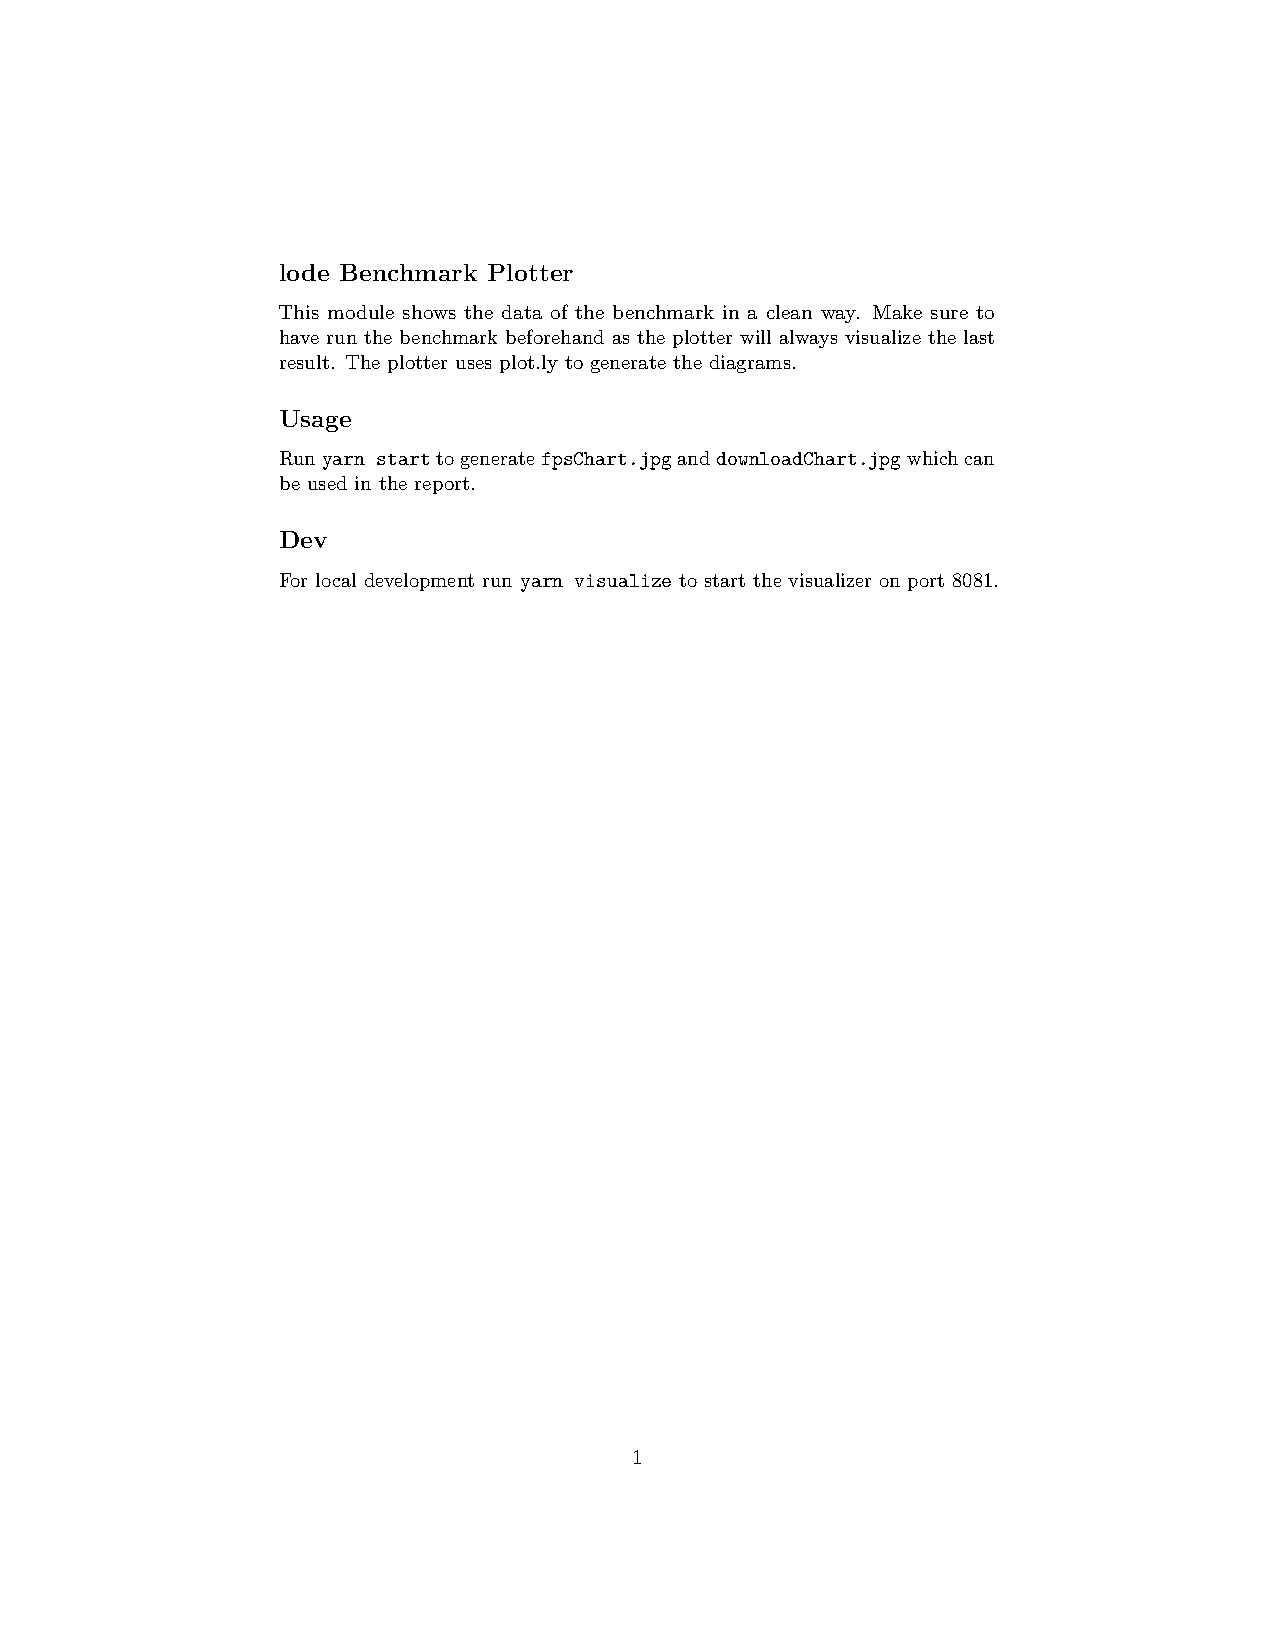
\includepdf[pagecommand={},scale=0.92,pages=-]{../ressources/packages/plotter.pdf}

\section{Benchmark Daten}
\begin{figure}[H]
  \begin{lstlisting}
optimized fps: 59.9 (0.316 standard deviation)
the value is with a confidence of 95% between 59.704 and 60.096
baseline fps: 48.3 (0.483 standard deviation)
the value is with a confidence of 95% between 48.001 and 48.599


further information for interpreting data:

gpuTotalTime:
optimized: 108.406 (5.667 standard deviation)
baseline: 336.718 (398.204 standard deviation)
medianRenderLoopDuration:
optimized: 2.067 (0.064 standard deviation)
baseline: 1.394 (0.024 standard deviation)
totalGpuEvents:
optimized: 524.7 (26.081 standard deviation)
baseline: 518.6 (17.89 standard deviation)
totalModelLoadDuration:
optimized: 1350.611 (42.677 standard deviation)
baseline: 1233.288 (53.571 standard deviation)
totalRenders:
optimized: 300.4 (5.602 standard deviation)
baseline: 232.3 (5.658 standard deviation)
  \end{lstlisting}
\caption{Durchlauf Benchmark auf MacBook Pro 2018}
\label{fig:marcbookBenchmarkRun}
\end{figure}

\begin{figure}[H]
  \begin{lstlisting}
    CPU: 2.9 GHz Quad-Core Intel Core i7
    GPU: Radeon Pro 560 4 GB
    RAM: 16 GB
  \end{lstlisting}
\caption{Hardwarespezifikation MacBook Pro 2018}
\label{fig:marcbookProSpecification}
\end{figure}

\begin{figure}[H]
  \begin{lstlisting}
optimized fps: 58.9 (0.316 standard deviation)
the value is with a confidence of 95% between 58.704 and 59.096
baseline fps: 11 (0.408 standard deviation)
the value is with a confidence of 95% between 10.747 and 11.253


further information for interpreting data:

gpuTotalTime:
optimized: 455.366 (139.317 standard deviation)
baseline: 174.948 (111.763 standard deviation)
medianRenderLoopDuration:
optimized: 2.448 (0.537 standard deviation)
baseline: 2.674 (0.603 standard deviation)
totalGpuEvents:
optimized: 490 (37.523 standard deviation)
baseline: 150.5 (11.326 standard deviation)
totalModelLoadDuration:
optimized: 1201.504 (167.149 standard deviation)
baseline: 1110.993 (140.091 standard deviation)
totalRenders:
optimized: 252.9 (56.432 standard deviation)
baseline: 56.8 (5.245 standard deviation)
  \end{lstlisting}
\caption{Durchlauf Benchmark auf Dell Precision 5540}
\label{fig:windowsBenchmarkRun}
\end{figure}

\begin{figure}[H]
  \begin{lstlisting}
CPU: 2.4 GHz Core Intel Core i9-9980HK
GPU: Intel UHD Graphics 630
RAM: 32 GB
  \end{lstlisting}
\caption{Hardwarespezifikation Dell Precision 5540}
\label{fig:windowsSpecification}
\end{figure}

\newpage

\section{Projektdokumentation}
\subsection{Zeitplan}
\begin{figure}[H]
  \centering
  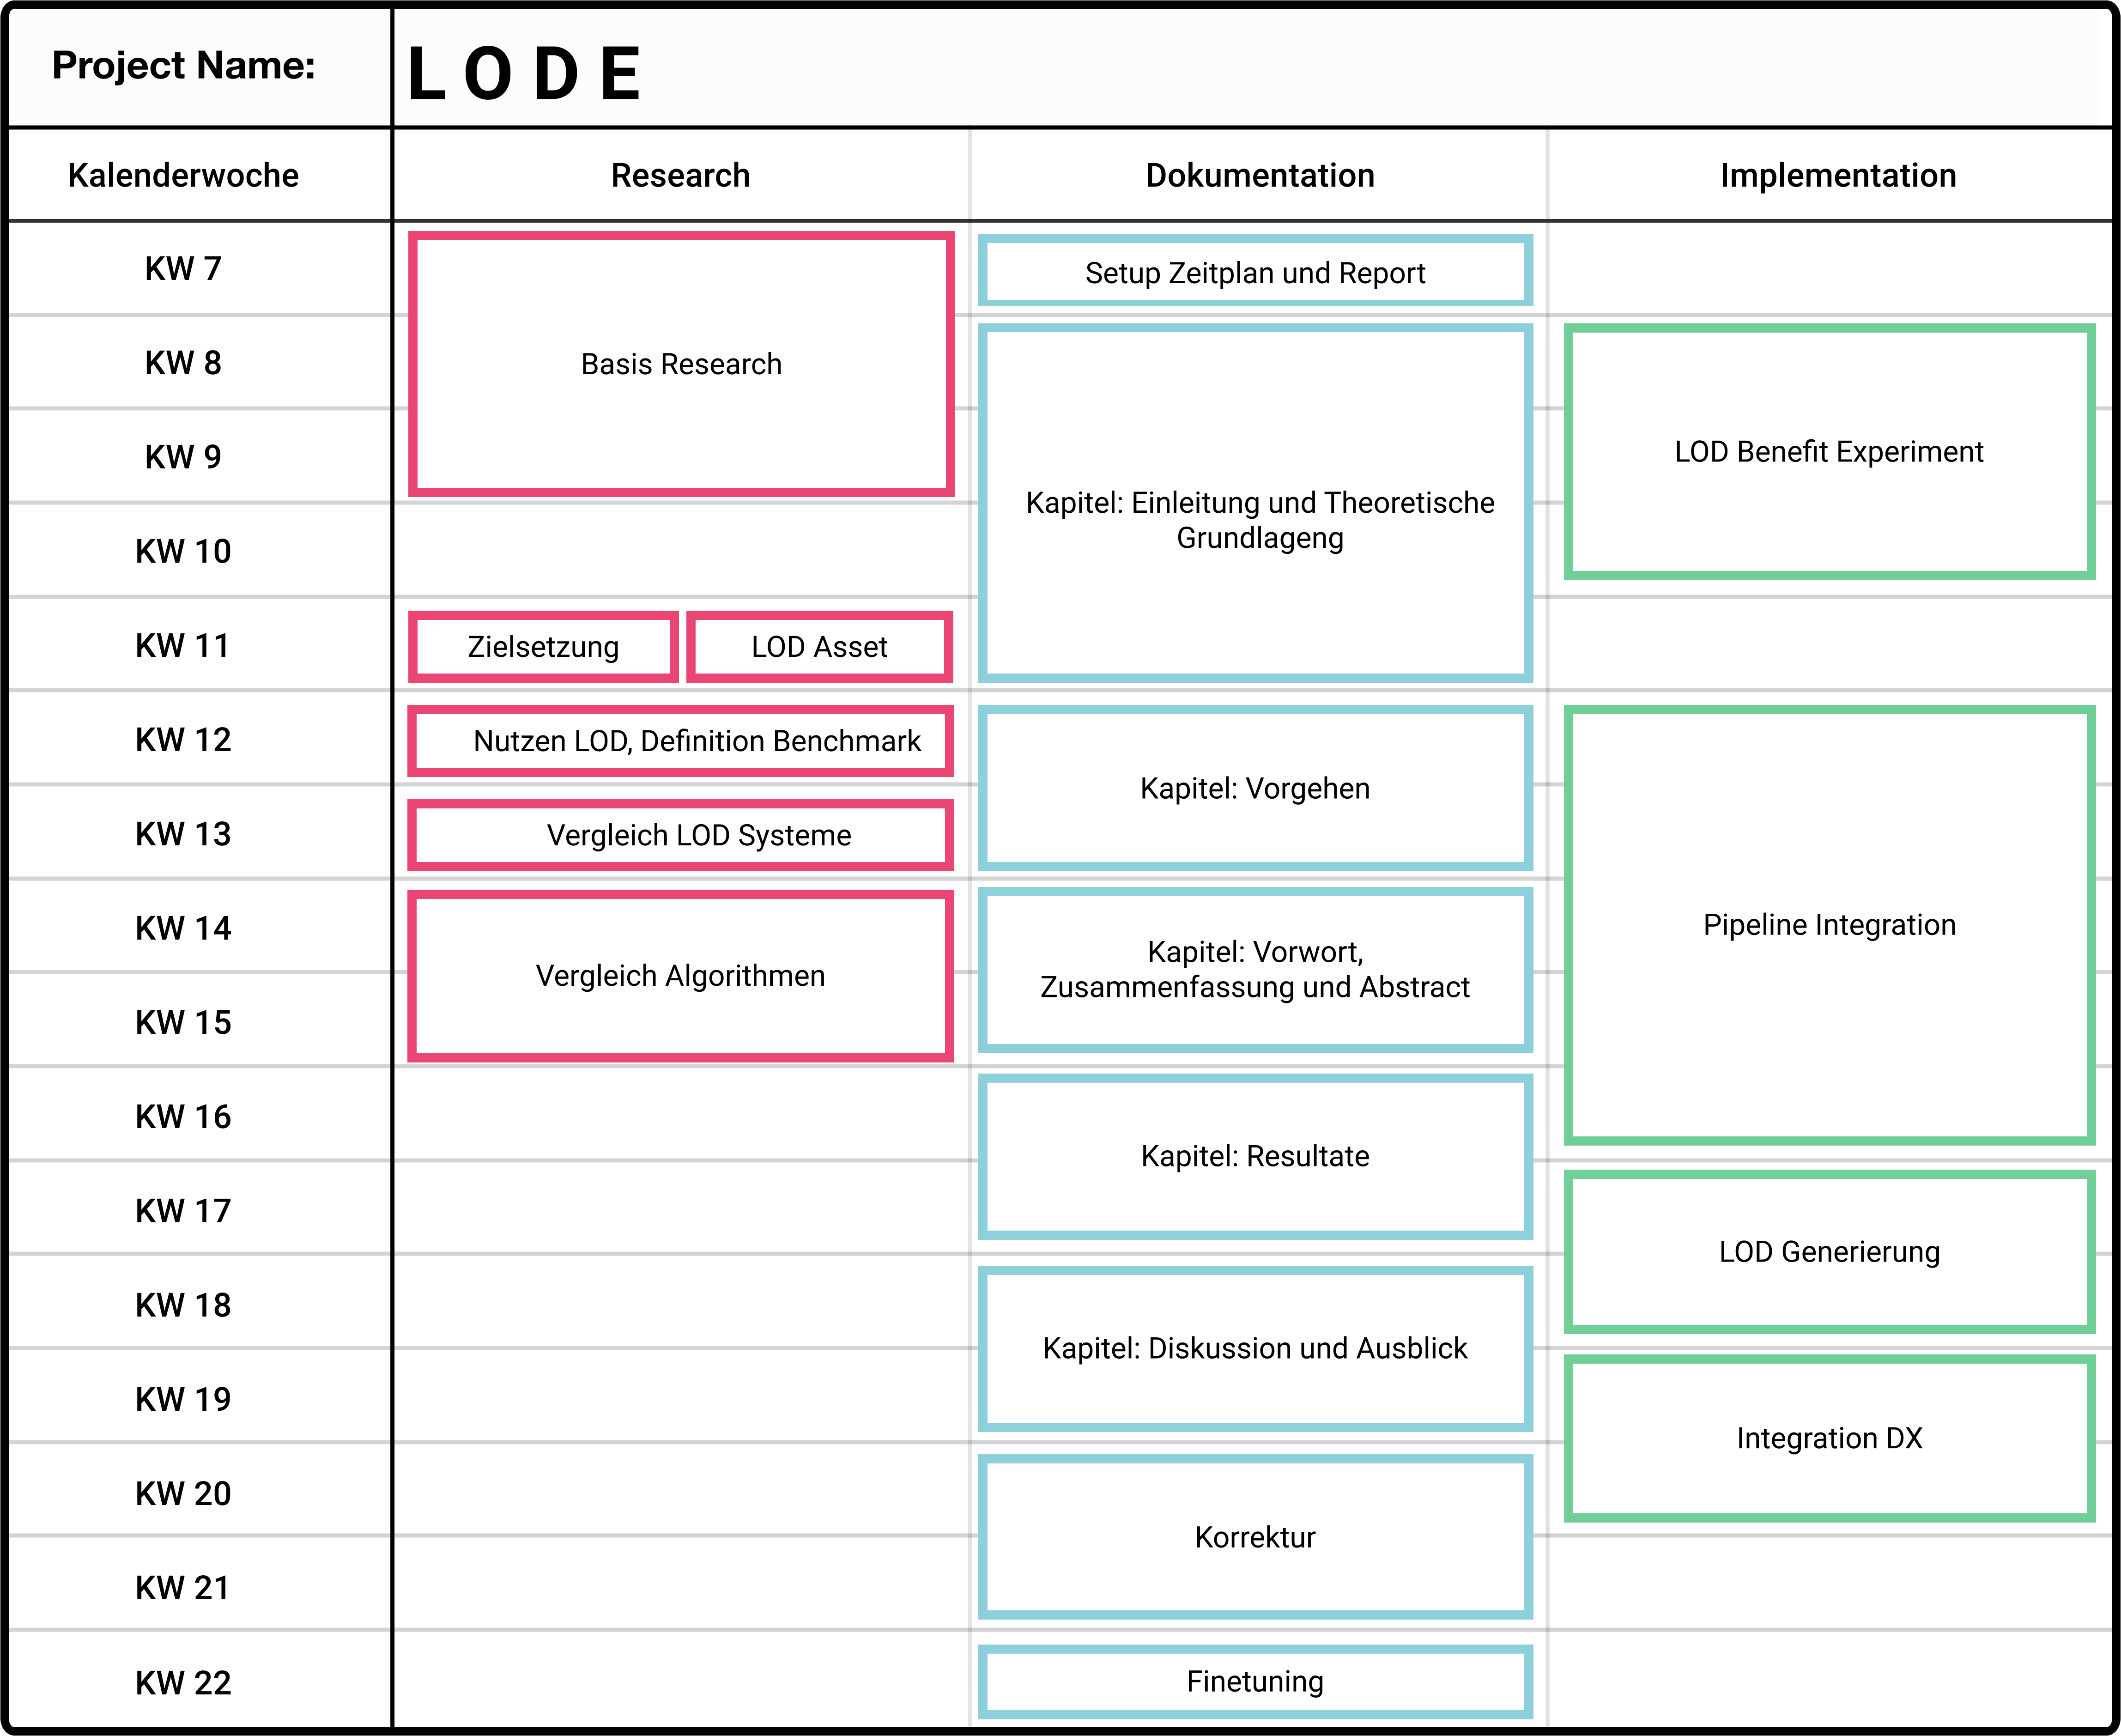
\includegraphics[width=1\columnwidth]{../ressources/zeitplan.png}
\end{figure}

\newpage

\subsection{Meeting-Protokolle}
\paragraph{21.05.2021}
Besprochenes:
\begin{itemize}
  \item Demo Szenerie finalisiert
  \item UI-Design für Lode-UI
  \item Bericht
  \item Basis Texturierung (Bsp. Ente)
\end{itemize}
Anmerkungen:
\begin{itemize}
  \item -
\end{itemize}
Geklärte Fragestellungen:
\begin{itemize}
  \item Titelanpassung möglich? -> Ja, “Pipeline” statt “Generierungs-System”: Level of Detail Pipeline für 3D-Webapplikationen
\end{itemize}
Offene Fragestellungen:
\begin{itemize}
  \item -
\end{itemize}
Nächste Schritte:
\begin{itemize}
  \item  Demoszenerie Fine-Tuning
  \item Fine-Tuning an Algorithmus
  \item Bericht
\end{itemize}

\newpage

\paragraph{14.05.2021}
Kein Meeting wegen Auffahrt.

\paragraph{07.05.2021}
Besprochenes:
\begin{itemize}
  \item Konfiguration per Level einstellbar
  \item Web-UI zur Levelkonfiguration
\end{itemize}
Anmerkungen:
\begin{itemize}
  \item Fokus auf Resultate im Bericht
\end{itemize}
Geklärte Fragestellungen:
\begin{itemize}
  \item -
\end{itemize}
Offene Fragestellungen:
\begin{itemize}
  \item Wann bekommen wir den Präsentationstermin? -> Noch nichts bekannt
\end{itemize}
Nächste Schritte:
\begin{itemize}
  \item Demo Szenerie fertigstellen
  \item UI-Design für Lode-UI
  \item Bericht
  \item Basis Texturierung (Bsp. Ente)
\end{itemize}

\newpage

\paragraph{30.04.2021}
Besprochenes:
\begin{itemize}
  \item Mehrere Levels (vom Benutzer einstellbar)
  \item GLTF Artefakten mit mehreren Meshs unterstützt
\end{itemize}
Anmerkungen:
\begin{itemize}
  \item -
\end{itemize}
Geklärte Fragestellungen:
\begin{itemize}
  \item Generelles zur Präsentation?
    \subitem Online
    \subitem Vier Personen: (Simon, Marc, Herr Burkert und Experte)
    \subitem Teilweise noch Studiengangleitung
    \subitem Zielpublikum: IT-Leute
\end{itemize}
Offene Fragestellungen:
\begin{itemize}
  \item -
\end{itemize}
Nächste Schritte:
\begin{itemize}
  \item Level-Wahl pro Modell
  \item Fine-Tune Webversion
  \item Demo Projekt dokumentieren
\end{itemize}

\newpage

\paragraph{23.04.2021}
Besprochenes:
\begin{itemize}
  \item Demo
  \item Pipielines
  \item Bericht
\end{itemize}
Anmerkungen:
\begin{itemize}
  \item Abstände um Fussnoten anschauen
  \item Ausgangslage noch breiter einsteigen (Inspiration von 2.1)
  \item Zwei Nomen nacheinander mit Bindestrich oder zusammenschreiben
  \item 2.4 könnte ausführlicher sein
  \item Graphics pipeline ausführlicher
  \item Generell: Möglichst viele Bilder, Beispiele und möglichst konkret
\end{itemize}
Geklärte Fragestellungen:
\begin{itemize}
  \item Gibt es Seiten Maximum? -> Nein, muss einfach alles Wichtige drinstehen
\end{itemize}
Offene Fragestellungen:
\begin{itemize}
  \item -
\end{itemize}
Nächste Schritte:
\begin{itemize}
  \item Zusammenfassung \& Vorwort schreiben
  \item Anzahl Level kann vom Benutzer angegeben werden
  \item CLI soll nur Modell generieren, die nicht bereits generiert sind
  \item LOD-Runtime als alleinstehendes Projekt zur Verfügung stellen
\end{itemize}

\newpage

\paragraph{16.04.2021}
Besprochenes:
\begin{itemize}
  \item Glossar mit Fussnoten
  \item Pipeline für Berichtgenerierung
  \item Algorithmus Prototyp läuft
\end{itemize}
Anmerkungen:
\begin{itemize}
  \item Glossar fehlt in Pipelinebuild
\end{itemize}
Geklärte Fragestellungen:
\begin{itemize}
  \item -
\end{itemize}
Offene Fragestellungen:
\begin{itemize}
  \item -
\end{itemize}
Nächste Schritte:
\begin{itemize}
  \item CLI Integration finalisieren
  \item OBJ Modelle suchen, die mit Algorithmus gut funktionieren
  \item CLI in Demoprojekt verwenden
  \item Demo Szenerie aufbauen mit Flyover
  \item DevExperience (Lode-Runtime)
  \item Algorithmus weitertreiben \& dokumentieren
\end{itemize}

\newpage

\paragraph{09.04.2021}
Besprochenes:
\begin{itemize}
  \item Algorithmus ausgesucht
  \item Datenformat auf glTF festgelegt
  \item Switch zu ThreeJS
  \item Setup deployment Pipeline
\end{itemize}
Anmerkungen:
\begin{itemize}
  \item -
\end{itemize}
Geklärte Fragestellungen:
\begin{itemize}
  \item Ähnliche bereits durchgeführte Berichte? -> Gibt es so nicht. Punktuelles Feedback statt Orientierungshilfe. Arbeit über functional GO [en] war gut – per Mail verschickt.
\end{itemize}
Offene Fragestellungen:
\begin{itemize}
  \item -
\end{itemize}
Nächste Schritte:
\begin{itemize}
  \item Bericht weitertreiben
  \item Pipeline fertig aufsetzen
  \item Algorithmus Prototyp zum Laufen bringen
\end{itemize}

\newpage

\paragraph{26.03.2021}
Besprochenes:
\begin{itemize}
  \item Bericht
    \subitem Quellen
  \item Benchmark
  \item CLI
\end{itemize}
Anmerkungen:
\begin{itemize}
  \item Benchmark
    \subitem Rahmenbedingungen festhalten
\end{itemize}
Geklärte Fragestellungen:
\begin{itemize}
  \item Glossareinträge jedes Mal referenzieren oder nur beim ersten Verwenden? -> Beim ersten Mal
  \item Glossareinträge beim ersten Verwenden direkt ebenfalls in die Fussnoten aufnehmen? -> Ja, guter Ansatz
\end{itemize}
Offene Fragestellungen:
\begin{itemize}
  \item -
\end{itemize}
Nächste Schritte:
\begin{itemize}
  \item Glossar / Emphasizing / Fussnoten
  \item Benchmark-Sektion in Report auf Akademisches-Level hieven
  \item Vergleich LOD System
  \item Anfang Auswahl LOD-Algorithmus
  \item Technischer Durchstich
  \item Switch von Babylon zu ThreeJs
  \item Github Pipeline und demo-host aufsetzen
\end{itemize}

\newpage

\paragraph{19.03.2021}
Besprochenes:
\begin{itemize}
  \item Bericht
  \item Zeitplan gezeigt und Abgrenzungen bestätigt
\end{itemize}
Anmerkungen:
\begin{itemize}
  \item Feedback Bericht Einleitung:
    \subitem Ausgangslage einstieg ein bisschen harsch
    \subitem Gross- / Kleinschreibung
  \item Feedback Bericht Grundlagen
    \subitem WebGL, WebGPU, OpenGL erklären
    \subitem Eventuell mit Fussnote oder Quellen verweise auf weiterführende Informationen
    \subitem Perpendikular -> Fussnote
    \subitem Mehr Beispiele (Visuell / Code)
    \subitem Transformations visuals ausgangs Bild jeweils links daneben anzeigen
    \subitem Frustum? -> Erklären
  \item Feedback Bericht Vorgehen
    \subitem Model erklären im Bericht
\end{itemize}
Geklärte Fragestellungen:
\begin{itemize}
  \item Sind Anglizismen OK? -> Ja, aber eventuell kursiv drucken
    \subitem Glossar aufbauen
  \item Sollen wir vermehrt auf Quellen setzen? -> Ja
\end{itemize}
Offene Fragestellungen:
\begin{itemize}
  \item -
\end{itemize}
Nächste Schritte:
\begin{itemize}
  \item Benchmark erweitern
  \item Bericht weitertreiben
  \item CLI aufsetzen
\end{itemize}

\newpage

\paragraph{12.03.2021}
Besprochenes:
\begin{itemize}
  \item Demo Projekt mit Benchmark
  \item Benchmarks nur mit Chrome getestet
  \item Verwendung von Puppeteer für Benchmark-tests
  \item Einleitung und Vorgehen Kapitel des Berichts
\end{itemize}
Anmerkungen:
\begin{itemize}
  \item Sieht so weit gut aus. Auf gutem Weg.
  \item Maximal 2/3 Seite Code-Ausschnitte
\end{itemize}
Geklärte Fragestellungen:
\begin{itemize}
  \item Hat Herr Burkert technische Grundlagen, um Projekt lokal laufen zu lassen? -> Ja.
  \item Sind Google interne Dokumente als Quellen zulässig? -> Ja, da öffentlich zugänglich. Weitere wissenschaftliche Quellen wünschenswert.
\end{itemize}
Offene Fragestellungen:
\begin{itemize}
  \item -
\end{itemize}
Nächste Schritte:
\begin{itemize}
  \item Herr Burkert gibt Feedback zu Detailierungsgrad des Berichts bis nächste Woche
  \item Herr Burkert schaut sich das Benchmark Projekt an und gibt erstes Feedback
  \item Zeitplan aktualisieren
  \item Simon und Marc geben Herrn Burkert ein Signal, wenn Bericht Inhaltlich bereit ist
  \item Alle Dokumente im Teams in den General Kanal verschieben
  \item In Zukunft Termine für Besprechungen aufsetzen.
\end{itemize}

\newpage

\paragraph{05.03.2021}
Besprochenes:
\begin{itemize}
  \item Gantt Chart (https://www.figma.com/file/8TcufkDndGDy1OalGoVVZP/Dokumentation-BA?node-id=1\%3A745)
  \item Report mit LaTeX: https://github.com/kreativwebdesign/lode/blob/main/documentation/report/doc.pdf
  \item Experiment zeigt Nutzen von LOD für mobile Geräte
\end{itemize}
Anmerkungen:
\begin{itemize}
  \item Ausführliche Einführung ins Thema LOD erwünscht (~15 Seiten)
  \item Meeting Protokolle im Teams erfassen
  \item Aufgabenstellung im Teams hochladen
  \item Demo im Bericht ausführlich beschreiben mit Bildern und Statistiken/Messungen
\end{itemize}
Geklärte Fragestellungen:
\begin{itemize}
  \item Muss Aufgabenstellung verfeinert werden? -> Nein, Highlevel gewährt uns Flexibilität
\end{itemize}
Offene Fragestellungen:
\begin{itemize}
  \item Gibt es einen einfachen weg, die GPU zu drosseln? -> Hardware abhängig, jedoch kann mit Chrome Dev Tools und Puppeteer im Headless Modus genügend detaillierte Informationen bzgl. GPU Leistung gefunden werden.
\end{itemize}
Nächste Schritte:
\begin{itemize}
  \item Einführung zum Thema LOD im Bericht schreiben
  \item Meeting nächsten Freitag 12.03. 13:00 Uhr um die erste Fassung der Einführung zu besprechen
\end{itemize}

\newpage

\paragraph{26.02.2021}
Besprochenes:
\begin{itemize}
  \item -
\end{itemize}
Anmerkungen:
\begin{itemize}
  \item -
\end{itemize}
Geklärte Fragestellungen:
\begin{itemize}
  \item Sprache? -> nur Deutsch
  \item Code öffentlich? -> auf Github (https://github.com/kreativwebdesign/lode)
  \item Relevanz Projektmanagement? -> Anhang
  \item Berichtstruktur? -> Details im Intranet
\end{itemize}
Offene Fragestellungen:
\begin{itemize}
  \item -
\end{itemize}
Nächste Schritte:
\begin{itemize}
  \item -
\end{itemize}
